\documentclass[dvipdfmx]{jsarticle}
\usepackage{penrosetensor}

\begin{document}

\section{記法一覧}
\label{sec: notation}

以下に掲げるのは本稿に登場した記法である.
本稿で登場した全ての記法は, 以下の記法の組み合わせである.
ここに掲載したもの以外にも\cite{boosting}などの等価な記法がある.

\begin{table}[h]
    \centering
    \begin{tabular}{ll}
        \toprule
        \parbox[c]{4zw}{スカラー}
        &
        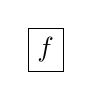
\begin{tikzpicture}
            \node at(0,0)[anchor=center, draw, rectangle]{$f$};
        \end{tikzpicture}
        \\
        \parbox[c]{6zw}{反変ベクトル}
        &
        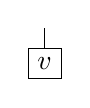
\begin{tikzpicture}
            \node at(0,0)[anchor=north, draw, rectangle](v){$\bm{v}$};
            \draw(v.north)--++(0,.25);
        \end{tikzpicture}
        \\
        \parbox[c]{6zw}{共変ベクトル}
        &
        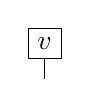
\begin{tikzpicture}
            \node at(0,0)[anchor=north, draw, rectangle](v){$\bm{v}$};
            \draw(v.south)--++(0,-.25);
        \end{tikzpicture}
        \\
        \parbox[c]{22zw}{反変2階共変3階テンソル}
        &
        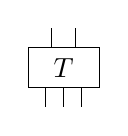
\begin{tikzpicture}
            \draw
                (0,0)rectangle(.9,.5)
                node at(.45,.25)[anchor=center](T){$T$}
                (.3,.5)--++(0,.25)
                (.6,.5)--++(0,.25)
                (.225,0)--++(0,-.25)
                (.45,0)--++(0,-.25)
                (.675,0)--++(0,-.25)
            ;
        \end{tikzpicture}
        \\
        \parbox[c]{20zw}{Kroneckerのデルタ$\delta_\mu^\nu$}
        &
        \begin{tikzpicture}
            \draw
                (0,0)--++(0,.25)
                .. controls ++(0,.25) and ++(0,-.25) .. ++(.25,.5)
                --++(0,.25)
            ;
        \end{tikzpicture}
        \\
        \parbox[c]{10zw}{計量テンソル$g^{\mu\nu}, g_{\mu\nu}$}
        &
        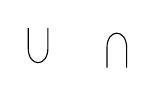
\begin{tikzpicture}
            \draw
                (0,0)--++(0,-.25)
                .. controls ++(0,-.25) and ++(0,-.25) .. ++(.25,0)
                --++(0,.25)
            ;
            \draw
                (1,-.5)--++(0,.25)
                .. controls ++(0,.25) and ++(0,.25) .. ++(.25,0)
                --++(0,-.25)
            ;
        \end{tikzpicture}
        \\
        \parbox[c]{22zw}{完全反対称Levi-Civitaテンソル$\epsilon_{\lambda\mu\cdots\nu}, \epsilon^{\lambda\mu\cdots\nu}$}
        &
        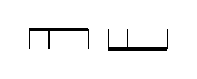
\begin{tikzpicture}
            \draw
                (0,0)--++(0,.25)
                (.25,0)--++(0,.25)
                (.75,0)--++(0,.25)
            ;
            \draw[very thick](0,.25)--(.75,.25);
            \draw
                (1,0)--++(0,.25)
                (1.25,0)--++(0,.25)
                (1.75,0)--++(0,.25)
            ;
            \draw[very thick](1,0)--(1.75,0);
        \end{tikzpicture}
        \\
        \parbox[c]{22zw}{反対称化操作}
        % \parbox[c]{22zw}{反対称化操作$\epsilon^{\lambda\mu\cdots\nu}_{\rho\sigma\cdots\tau}$}
        &
        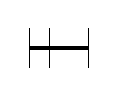
\begin{tikzpicture}
            \draw
                (0,-.25)--++(0,.5)
                (.25,-.25)--++(0,.5)
                (.75,-.25)--++(0,.5)
            ;
            \draw[ultra thick](0,0)--(.75,0);
            % \draw
            %     (0,-.25)--++(0,.5)node[above]{$\lambda$}
            %     (.25,-.25)--++(0,.5)node[above]{$\mu$}
            %     (.75,-.25)--++(0,.5)node[above]{$\nu$}
            % ;
            % \node at(0,-.25)[anchor=north]{$\rho$};
            % \node at(.25,-.25)[anchor=north]{$\sigma$};
            % \node at(.75,-.25)[anchor=north]{$\tau$};
        \end{tikzpicture}
        \\
        \parbox{10zw}{対称化操作}
        &
        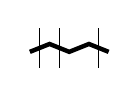
\begin{tikzpicture}
            \draw
                (0,-.25)--++(0,.5)
                (.25,-.25)--++(0,.5)
                (.75,-.25)--++(0,.5)
            ;
            \draw[ultra thick]
                (-.125,-.05)--(.125,.05)
                --(.375,-.05)
                --(.625,.05)
                --(.875,-.05)
            ;
        \end{tikzpicture}
        \\
        \parbox[c]{10zw}{共変微分$\nabla$}
        &
        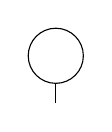
\begin{tikzpicture}
            \draw(0,0)circle[radius=.35];
            \draw(0,-.35)--++(0,-.25);
        \end{tikzpicture}
        \\
        \bottomrule
    \end{tabular}
\end{table}

\end{document}
